\section{Task Definition}
\label{sec:task}

We formally define the graph classification problem and establish notation for the five-model comparison used throughout the paper. Rather than changing many components at once, we keep the graph classification setting fixed and study how different residual information-flow mechanisms affect graph-level prediction under a common formulation.

\subsection{Graph Representation and Notation}

Let $\mathcal{G} = (\mathcal{V}, \mathcal{E})$ denote an undirected or directed graph, where $\mathcal{V} = \{v_1, v_2, \ldots, v_n\}$ is the set of $n$ nodes and $\mathcal{E} \subseteq \mathcal{V} \times \mathcal{V}$ is the set of edges. Each node $v_i \in \mathcal{V}$ is associated with a feature vector $\mathbf{x}_i \in \mathbb{R}^{d_{\text{in}}}$, where $d_{\text{in}}$ is the input feature dimension. The node features for the entire graph are collected in a matrix $\mathbf{X} \in \mathbb{R}^{n \times d_{\text{in}}}$, where the $i$-th row corresponds to $\mathbf{x}_i$.

The graph structure is represented using an adjacency matrix $\mathbf{A} \in \{0,1\}^{n \times n}$, where $A_{ij} = 1$ if there exists an edge $(v_i, v_j) \in \mathcal{E}$, and $A_{ij} = 0$ otherwise. For undirected graphs, the adjacency matrix is symmetric ($\mathbf{A} = \mathbf{A}^\top$). Optionally, edge features can be represented as $\mathbf{e}_{uv} \in \mathbb{R}^{d_e}$ for each edge $(u,v) \in \mathcal{E}$, or collected in a tensor $\mathbf{E} \in \mathbb{R}^{n \times n \times d_e}$.

\subsection{Graph Classification Problem}

Given a training dataset $\mathcal{D} = \{(\mathcal{G}_i, y_i)\}_{i=1}^{N}$ consisting of $N$ graphs, where each graph $\mathcal{G}_i$ is associated with a label $y_i \in \mathcal{Y}$, our objective is to learn a mapping function $f_\theta: \mathcal{G} \rightarrow \hat{y}$ that predicts the label $\hat{y} \in \mathcal{Y}$ for an unseen graph. The label space $\mathcal{Y}$ depends on the task type:
\begin{itemize}
    \item \textbf{Binary classification}: $\mathcal{Y} = \{0, 1\}$ (e.g., molecular toxicity prediction)
    \item \textbf{Multi-class classification}: $\mathcal{Y} = \{1, 2, \ldots, C\}$ (e.g., graph categorization into $C$ classes)
    \item \textbf{Multi-label classification}: $\mathcal{Y} \subseteq \{1, 2, \ldots, C\}$ (e.g., a graph may belong to multiple categories simultaneously)
\end{itemize}

The function $f_\theta$ is parameterized by neural network weights $\theta$ and operates by first learning node-level representations through message passing, then aggregating these into a graph-level representation, and finally mapping this representation to the output label space.

\subsection{Main Comparison Setting}

The main paper compares five architectures under the same graph-classification pipeline:
\begin{itemize}
    \item \textbf{PlainGNN}: sequential message passing without explicit state reuse
    \item \textbf{NodeResGNN}: single-branch node-level residual reuse
    \item \textbf{NodeCrossGNN}: two-branch node-level cross exchange
    \item \textbf{GraphResGNN}: graph-level residual propagation across sequential blocks
    \item \textbf{GraphCrossGNN}: graph-level cross-summary exchange across paired blocks
\end{itemize}

The comparison is designed to isolate \emph{where} information is reused: inside one branch, across parallel branches, or through pooled graph summaries passed between blocks. This design makes the main experimental question precise: when does cross-path interaction help beyond plain stacking and beyond a simpler residual baseline?

\begin{figure}[t]
\centering
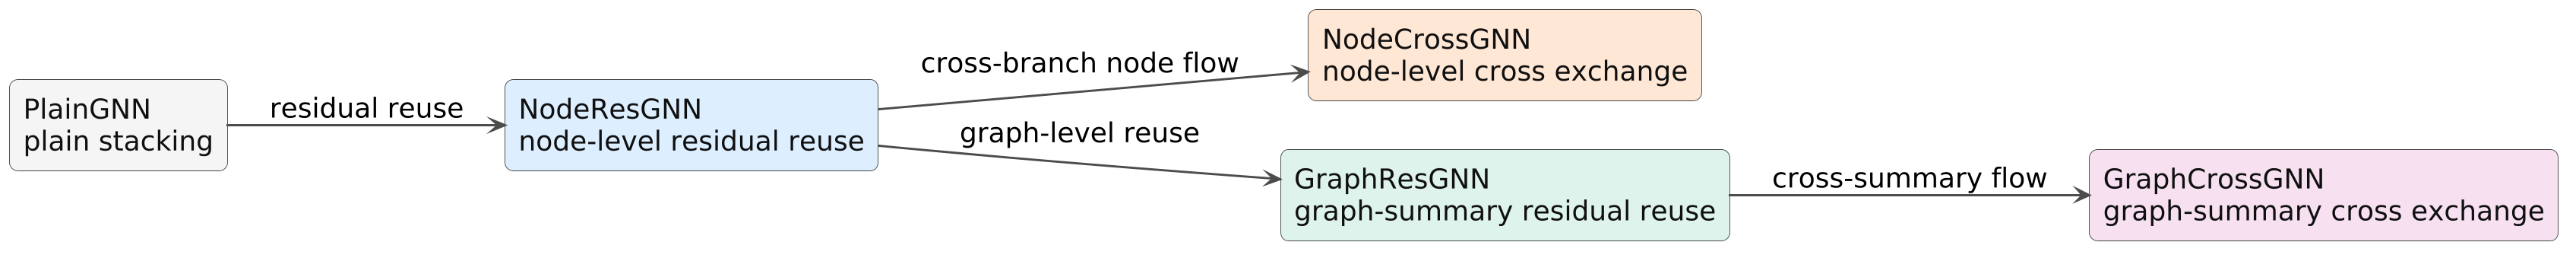
\includegraphics[width=0.98\linewidth]{figures/task_model_comparison.png}
\caption{Main model comparison in this paper. The five architectures differ only in how intermediate node states or graph summaries are reused, which allows a controlled study of residual and cross-residual information flow.}
\label{fig:task_model_comparison}
\end{figure}

\subsection{Message Passing with Multiple Operators}

Let $\Phi$ denote a message-passing operator. For a chosen backbone, node representations are updated over $L$ layers. At layer $\ell$, the representation $\mathbf{h}_i^{(\ell)}$ of node $v_i$ is computed as:

\begin{equation}
\mathbf{h}_i^{(\ell+1)} = \sigma\left(\mathbf{W}^{(\ell)} \cdot \text{AGGREGATE}_{\Phi}\left(\left\{\mathbf{h}_j^{(\ell)} : j \in \mathcal{N}(i)\right\}, \mathbf{h}_i^{(\ell)}\right) + \mathbf{b}^{(\ell)}\right)
\end{equation}

where $\text{AGGREGATE}_{\Phi}$ is the aggregation function induced by $\Phi$, $\mathbf{W}^{(\ell)}$ and $\mathbf{b}^{(\ell)}$ are learnable parameters, and $\sigma$ is a non-linear activation function. In the experiments reported later, all five models are compared under the same GCN-style backbone so that the observed differences are attributable to information-flow design rather than to operator changes.

\subsection{Graph-Level Representation Learning}

After $L$ layers of message passing, a readout function $R$ aggregates node-level representations into a graph-level embedding $\mathbf{h}_{\mathcal{G}} \in \mathbb{R}^{d_{\text{out}}}$:

\begin{equation}
\mathbf{h}_{\mathcal{G}} = R\left(\left\{\mathbf{h}_i^{(L)} : i = 1, \ldots, n\right\}\right)
\end{equation}

Common readout functions include mean, max, and sum pooling. In our framework, graph-level representations may also be reused across successive computation blocks, enabling later stages to incorporate coarse whole-graph context in addition to local message-passing features.

\subsection{Learning Objective}

The graph-level representation is passed through a classifier (typically a linear layer followed by softmax) to produce the predicted label distribution:

\begin{equation}
\hat{\mathbf{y}} = \text{softmax}\left(\mathbf{W}_{\text{clf}} \mathbf{h}_{\mathcal{G}} + \mathbf{b}_{\text{clf}}\right)
\end{equation}

where $\hat{\mathbf{y}} \in \mathbb{R}^{C}$ (for multi-class classification) is the predicted probability distribution over $C$ classes, and $\mathbf{W}_{\text{clf}} \in \mathbb{R}^{C \times d_{\text{out}}}$, $\mathbf{b}_{\text{clf}} \in \mathbb{R}^{C}$ are classifier parameters.

The model is trained end-to-end by minimizing the cross-entropy loss function:

\begin{equation}
\mathcal{L}(\theta) = -\frac{1}{N} \sum_{i=1}^{N} \sum_{c=1}^{C} y_{i,c} \log(\hat{y}_{i,c})
\end{equation}

where $y_{i,c} \in \{0, 1\}$ is the ground-truth label indicator (one-hot encoding) for graph $\mathcal{G}_i$ and class $c$, and $\hat{y}_{i,c}$ is the predicted probability for class $c$. For binary classification, this reduces to the binary cross-entropy loss. With this common formulation fixed, the next section instantiates the five CR-GNN variants and specifies how each one reuses intermediate node states or graph summaries.
